\chapter{Ground states, symmetries, and defects}\label{chap: ground-states}
In this chapter we investigate the ground states of spinor BECs obtained through
minimizing the corresponding mean-field energy functional.
In particular, we investigate the symmetry properties using both Majorana and
spherical harmonic representations.
Furthermore, we construct the phase diagrams for conserved and non-conserved
magnetisation.
Finally, we construct some topological defects present in these systems.

There are numerous references (e.g., see~\cite{Ciobanu2000, Zhang2003,
    Kawaguchi2012, StamperKurn2013}) that already provide most of these results,
but we reproduce them here to provide reference for subsequent chapters.
Furthermore, there are subtleties between the phase diagrams of spinor BECs
in the presence of conserved magnetisation that is not widely reported, so we
construct both phase diagrams (conserved and non-conserved) here to clarify
distinctions between the two.


\section{Spin-1}\label{sec: ground-states-spin-1}

\subsection{Ground states in a uniform system}

For a spin-1 system, the interacting part of the energy functional contains
two independent non-linear interaction terms (see
Sec.~\ref{subsec: spin-1-int-hamil}), given by
\begin{equation}
    E_\mathrm{int} = \frac{1}{2}\int c_0n^2+c_1|\vb{F}|^2 d\vb{r}.
\end{equation}
Since the density term remains fixed for a given normalised ground state, the
spin magnitude is the only relevant term.

For ferromagnetic interactions (\(c_1 < 0 \)), the energy is minimised when
the spin magnitude is maximised, i.e., \(|\vb{F}| = n\).
A representative spinor for a ferromagnetic ground state is then
\begin{equation}
    \zeta^\mathrm{FM} = \mqty(1 \\ 0 \\ 0).
\end{equation}

In the absence of a magnetic field, the energy of a given spinor is degenerate
with respect to a global \(U(1)\) phase \(e^{i\theta}\) and an \(SO(3)\) spin
rotation, parameterized by three Euler angles \(\alpha, \beta \),
and \(\gamma \).
A general spin rotation represents rotations around the \(z-y-z\) axes:
\(U(\alpha, \beta, \gamma) = e^{-i\alpha F_z}e^{-i\beta F_y}e^{-i\gamma F_z}\).
In explicit matrix form, this becomes
\begin{equation}
    U(\alpha, \beta, \gamma) = \mqty(
    e^{-i(\alpha + \gamma)}\cos^2\frac{\beta}{2} &
    -\frac{e^{-i\alpha}}{\sqrt{2}}\sin\beta &
    e^{-i(\alpha - \gamma)}\sin^2\frac{\beta}{2} \\
    \frac{e^{-i\gamma}}{\sqrt{2}}\sin\beta &
    \cos\beta &
    -\frac{e^{i\gamma}}{\sqrt{2}}\sin\beta \\
    e^{i(\alpha - \gamma)}\cos^2\frac{\beta}{2} &
    \frac{e^{i\alpha}}{\sqrt{2}}\sin\beta &
    e^{i(\alpha + \gamma)}\sin^2\frac{\beta}{2}
    ).
\end{equation}

The general ferromagnetic wave function is constructed by
\begin{equation}\label{eq: FM-representative-spinor}
    \psi^\mathrm{FM} =
    \sqrt{n}e^{i\theta}U(\alpha, \beta, \gamma)\zeta^\mathrm{FM} =
    \sqrt{n}e^{i(\theta - \gamma)}\mqty(
    e^{-i\alpha}\cos^2\frac{\beta}{2} \\
    \frac{1}{\sqrt{2}}\sin\beta \\
    e^{i\alpha}\sin^2\frac{\beta}{2}
    ).
\end{equation}

For polar interactions (\(c_1 > 0\)), the energy is minimised by having the
spin magnitude vanish \(|F|=0\).
A representative polar spinor is
\begin{equation}\label{eq: EAP-spinor}
    \zeta^\mathrm{P} = \mqty(0 \\ 1 \\ 0).
\end{equation}
Similar to the FM case, a general polar wave function is given by
\begin{equation}\label{eq: polar-representative-spinor}
    \psi^\mathrm{P} =
    \sqrt{n}e^{i\theta}U(\alpha, \beta, \gamma)\zeta^\mathrm{P} =
    \sqrt{n}e^{i\theta}\mqty(
    -\frac{e^{-i\alpha}}{\sqrt{2}}\sin\beta \\
    \cos\beta \\
    \frac{e^{i\alpha}}{\sqrt{2}}\sin\beta
    ).
\end{equation}

Thus, in the absence of a magnetic field, there are two ground states in a
spin-1 system: polar and ferromagnetic, depending on the sign of the
spin-dependent interaction term, \(c_1\).

The presence of an external magnetic field drastically changes the valid ground
states of the spin-1 system.
\begin{figure}[htb]
    \centering
    \begin{tikzpicture}
        \node[anchor=south west, inner sep=0] (sodium) at (0, 0)
        {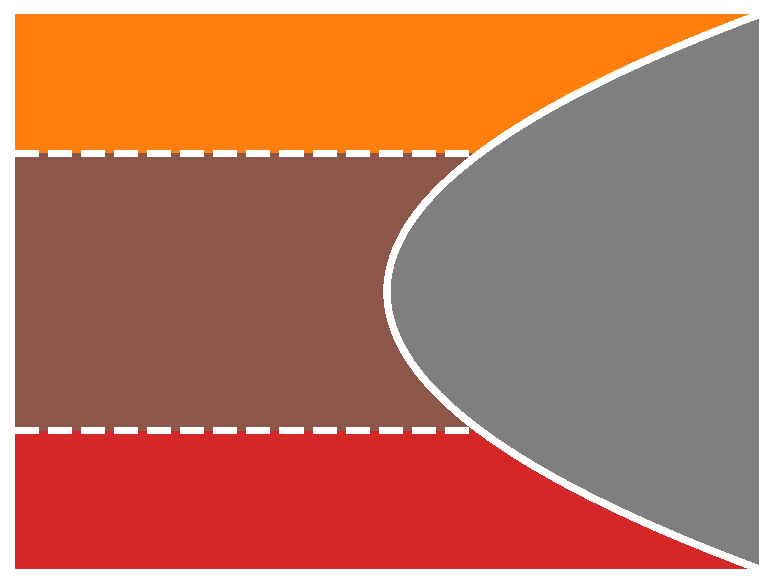
\includegraphics[width=0.38\textwidth]
            {gfx/ch-groundStateSymmetries/ground_states_polar_int_spin1.pdf}};
        \node[anchor=south west, inner sep=0] (rubidium) at (8, 0)
        {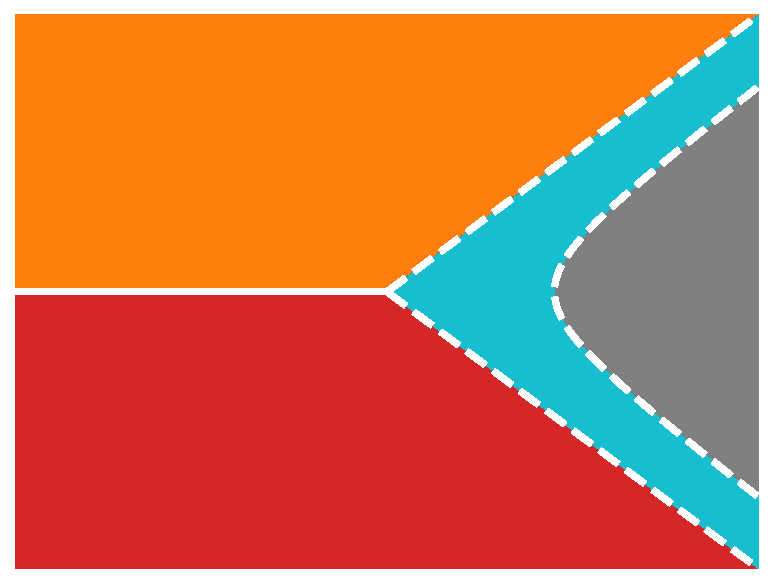
\includegraphics[width=0.38\textwidth]
            {gfx/ch-groundStateSymmetries/ground_states_fm_int_spin1.pdf}};

        \begin{scope}[x={($0.1*(sodium.south east)$)},
                y={($0.1*(sodium.north west)$)}]
            \draw[->, thick] (0,5)--(10.3,5) node[right]{$\frac{q}{c_1n}$};
            \draw[->, thick] (4.97,0)--(4.97,10.3) node[above]{$\frac{p}{c_1n}$};
            \draw[-] (6.1, 4.8) -- (6.1, 5.2);
            \node[anchor = south west] at (6.5, 3)
            {\scriptsize $p^2=2c_1nq$};
            \draw[->, thick] (6.6, 3.1) -- (6.25,2.55);
            \node at (4.8, 7.75) {\scriptsize $1$};
            \node at (4.7, 2.25) {\scriptsize -$1$};
            \node at (6.1, 4.5) {\scriptsize 1/2};
            \node[anchor=south west] at (0.5, 8.2)
            {\textcolor{white}{Ferromagnetic (I)}};
            \node[anchor=south west] at (0.5, 0.5)
            {\textcolor{white}{Ferromagnetic (II)}};
            \node[anchor=south west] at (0., 4.9)
            {\textcolor{white}{\small Antiferromagnetic}};
            \node[anchor=south west] at (2.1, 3.8)
            {\textcolor{white}{(III)}};
            \node[anchor=south west] at (6.5, 4.9)
            {\textcolor{white}{Polar (IV)}};
            \node[anchor=south west] at (3.8, -1.5) {\large $c_1 > 0$};
        \end{scope}
        \begin{scope}[x={($0.1*(sodium.south east)$)},
                y={($0.1*(sodium.north west)$)}]
            \draw[->, thick] (19.3,5)--(24.5,5) node[right]{$\frac{q}{|c_1|n}$};
            \draw[->, thick] (19.3,0)--(19.3,10.3) node[above]
            {$\frac{p}{|c_1|n}$};
            \node[anchor=south west] at (19.2, 8.6)
            {\scriptsize $p^2=q^2-2|c_1|nq$};
            \draw[->, thick] (19.7, 8.8) -- (21.9, 6.2);
            \node[anchor=south west, inner sep=0, rotate=-38] at (19.3, 4.)
            {\scriptsize $p=-q$};
            \node[anchor=south west, inner sep=0, rotate=38] at (19.5, 5.3)
            {\scriptsize $p=q$};
            \node[anchor=south west, inner sep=0] at (21.7, 4.5)
            {\scriptsize $2$};
            \node[anchor=south west] at (14.8, 6.5)
            {\textcolor{white}{Ferromagnetic (I)}};
            \node[anchor=south west] at (14.8, 1.5)
            {\textcolor{white}{Ferromagnetic (II)}};
            \node[anchor=south west] at (20.1, 4.9)
            {\textcolor{white}{BA}};
            \node[anchor=south west] at (20.1, 3.8)
            {\textcolor{white}{(V)}};
            \node[anchor=south west] at (22.1, 4.9)
            {\textcolor{white}{Polar}};
            \node[anchor=south west] at (22.1, 3.8)
            {\textcolor{white}{(IV)}};
            \node[anchor=south west] at (18., -1.5) {\large $c_1 < 0$};
        \end{scope}
    \end{tikzpicture}
    \caption[Spin-1 ground state phase diagram]
    {\label{fig: GS-phase-diagram}Ground state phase diagrams of spin-1
        BECs for polar (\(c_1 > 0\)) and ferromagnetic (\(c_1 < 0\))
        interactions in a parameter space of \((p, q)\).
        Solid or dashed white lines represent discontinuous and continuous phase
        transitions, respectively.}
\end{figure}
Fig.~\ref{fig: GS-phase-diagram} shows the ground state phase diagram for spin-1
BECs with \(c_1 > 0\) (left) and \(c_1 < 0\) (right) in the presence of a
magnetic field.
The full derivation of the ground state phase diagram can be found in recent
reviews~\cite{Kawaguchi2012, StamperKurn2013}.
There are five total ground states shown in Fig.~\ref{fig: GS-phase-diagram},
which are summarised in Table~\ref{tab: spin-1-ground-states}.
\begin{table}
    \centering
    \begin{tabular}{ccc}
        \toprule
        Ground state                          & Spinor, \(\zeta^T\)                      & \(F_z\) \\
        \midrule
        Ferromagnetic (I)                     & \((1, 0, 0)\)                            & 1       \\
        Ferromagnetic (II)                    & \((0, 0, 1)\)                            & -1      \\
        Antiferromagnetic (III)               & \(\left(\sqrt{\frac{1 + p(c_1n)}{2}}, 0,
        \sqrt{\frac{1 - p(c_1n)}{2}}\right)\) & \(\frac{p}{c_1n}\)                                 \\
        Polar (IV)                            & \((0, 1, 0)\)                            & 0       \\
        Broken-axisymmetry (V)                & Eq.~\eqref{eq: BA-spinor}
                                              & \(\frac{p(-p^2+q^2+2qc_1n)}{2c_1nq^2}\)            \\
        \bottomrule
    \end{tabular}
    \caption{\label{tab: spin-1-ground-states}Summary of the ground state
        phases in a spin-1 BEC with their respective spinors and magnetisation.}
\end{table}

There exists a fully magnetised ferromagnetic state with \(\zeta={(1, 0, 0)}^T\)
and \(F_z=1\) (state I) or \(\zeta={(0, 0, 1)}^T\) and \(F_z=-1\) (state II),
depending on the sign of the linear Zeeman shift \(p\).

For polar interactions \(c_1 > 0\), there exists an antiferromagnetic phase
(state III) with
\begin{equation}\label{eq: AFM-spinor}
    \zeta^\mathrm{AFM} = {\left(\sqrt{\frac{1 + p/(c_1n)}{2}}, 0,
    \sqrt{\frac{1 - p/(c_1n)}{2}}\right)}^T,
\end{equation}
and \(F_z = p/(c_1n)\).

A non-magnetised polar phase (state IV) arises with \(\zeta={(0, 1, 0)}^T\) and
\(F_z = 0\).

Finally, a broken-axisymmetry (BA) phase (state V) occurs in a condensate with
ferromagnetic interactions that has the form
\begin{equation}
    \begin{aligned}
        \zeta_{\pm 1} & =
        \frac{q \pm p}{2q}\sqrt{\frac{-p^2+q^2+2c_1nq}{2c_1nq}},              \\
        \zeta_0       & = \sqrt{\frac{(q^2-p^2)(-p^2-q^2+2c_1nq)}{4c_1nq^3}},
    \end{aligned}
    \label{eq: BA-spinor}
\end{equation}
which has a magnetisation that tilts against the quantisation axis
\begin{equation}
    F_z = \frac{p(-p^2 + q^2 + 2qc_1n)}{2c_1nq^2}.
\end{equation}
These five ground states fully encapsulate the phase diagram of spin-1 BECs
in a magnetic field.

\subsection{Graphical representation}
To visualise the symmetries of ground states it is useful to define graphical
representations.
The first to consider is the spherical harmonic, which maps the order parameter
onto spherical harmonics using the relation
\begin{equation}
    \Psi(\hat{s}) = \sum_m\psi_m Y_f^m(\hat{s}),
    \label{eq: spherical-harmonics}
\end{equation}
where \(\hat{s}\) is a unit vector in 3D spin space, and \(Y_f^m \) are the
spherical harmonics for a spin-\(f\) state.
The symmetry can be visualised with a surface plot of \(|\Psi(\hat{s})|^2\),
where the surface colour is represented by the argument of \(\Psi(\hat{s})\).

The orientation of the spherical harmonics corresponds to the condensate spin,
and so as the spin vector rotates, the orientation of spherical harmonics
rotates to match.
In addition, the colour of the spherical harmonics corresponds to the global
phase, \( \theta \).
Therefore, the spherical harmonics give an accurate description of the
physical symmetries of the wave function, along with a pictorial representation
of how the phase is changing.
Throughout this thesis we will use the spherical harmonics to construct a
picture of what is happening to the wave function at different locations in
space, where the symmetry of the wave function can rapidly transform in a
non-trivial manner.

In spin-1, there are three \(f = 1\) spherical harmonics given by
\begin{align}
    Y_1^0(\theta, \phi)       & = \frac{1}{2}\sqrt{\frac{3}{\pi}}\cos\theta, \\
    Y_1^{\pm 1}(\theta, \phi) & =
    \frac{1}{2}\sqrt{\frac{3}{2\pi}}e^{\pm i \phi}\sin\theta.
\end{align}
The spherical harmonic representations of the spin-1 polar and ferromagnetic
ground states are shown in Fig.~\ref{fig: spin-1-spherical-harmonics}.
\begin{figure}
    \begin{tikzpicture}
        % Plots
        \node at (0, 0) {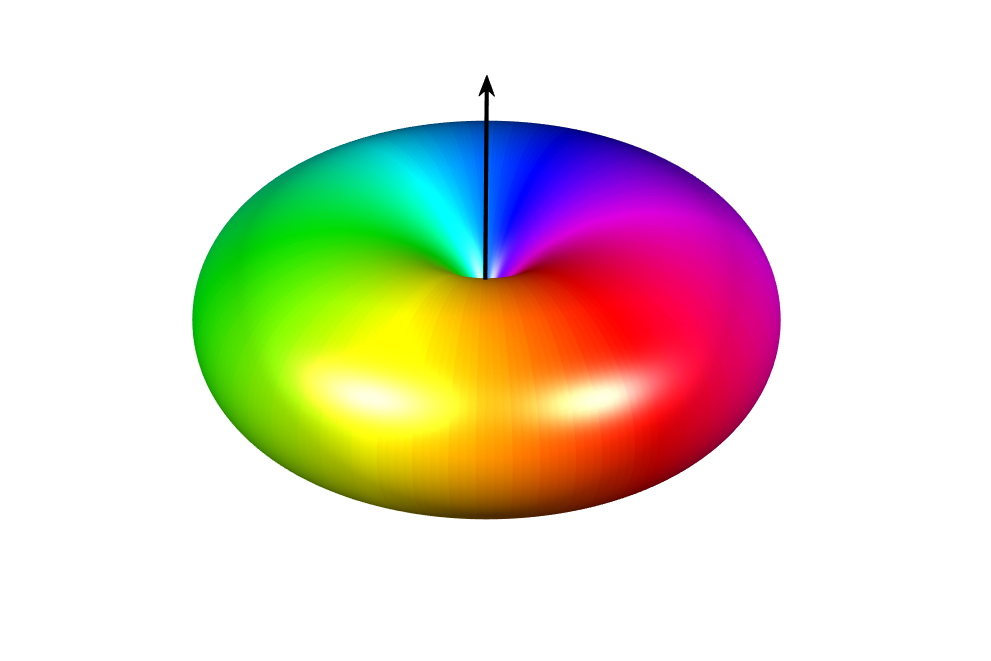
\includegraphics[width=0.49\textwidth]
            {gfx/ch-groundStateSymmetries/FM-spherical.pdf}};
        \node at (7.2, 0) {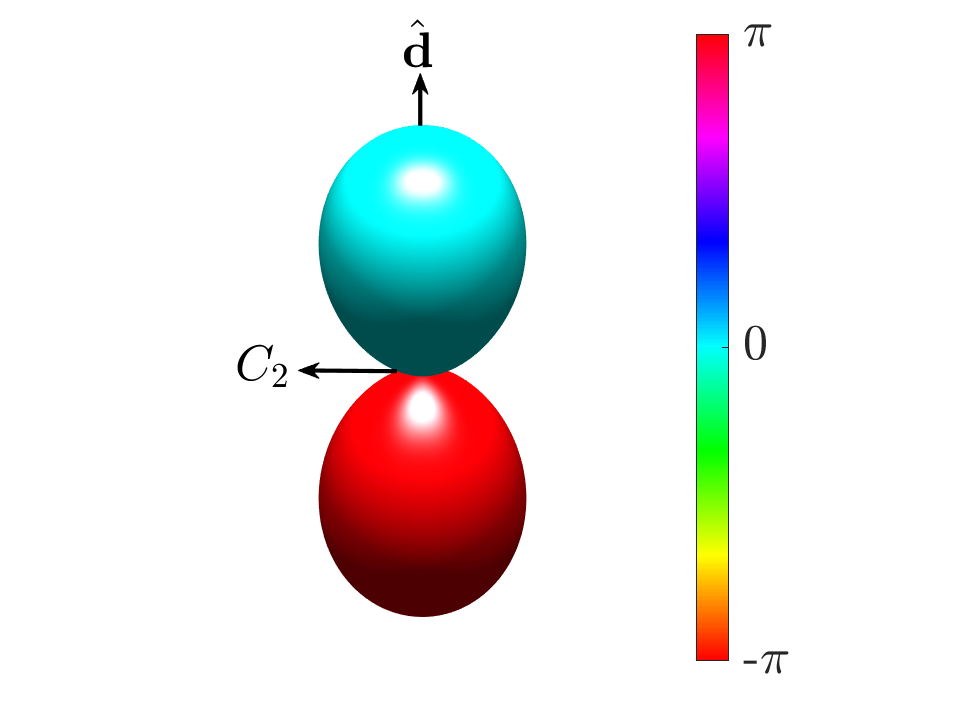
\includegraphics[scale=0.55]
            {gfx/ch-groundStateSymmetries/polar-spherical.pdf}};
        \node at (0, -5) {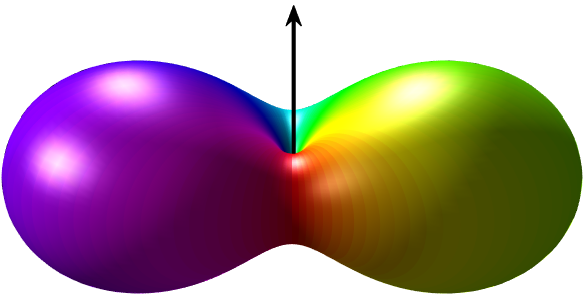
\includegraphics[width=0.49\textwidth]
            {gfx/ch-groundStateSymmetries/AFM-spherical.pdf}};
        \node at (7.2, -5) {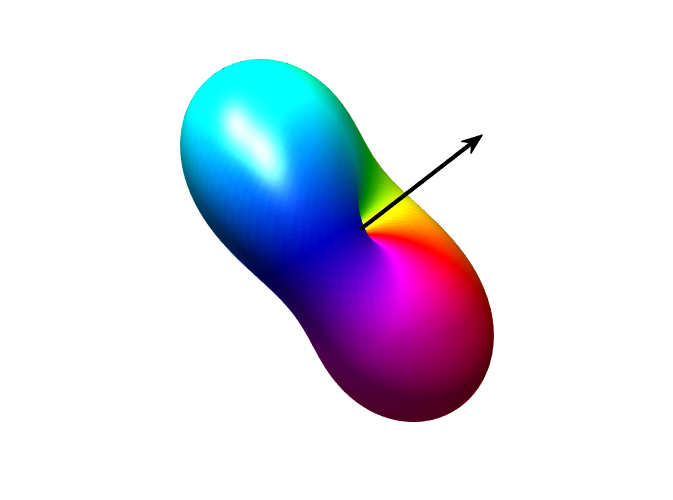
\includegraphics[width=0.49\textwidth]
            {gfx/ch-groundStateSymmetries/BA-spherical.pdf}};

        % Colour bar
        \node at (4, 0) {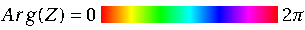
\includegraphics[angle=90]
            {gfx/colourbars/compiled_hsv.pdf}};

        % Labels
        \node at (0, -2.) {(a)};
        \node at (7.2, -2.) {(b)};
        \node at (0, -7.2) {(c)};
        \node at (7.2, -7.2) {(d)};

        % Spinors
        \node at (0, 3) {\(\zeta^\mathrm{FM}={(1, 0, 0)}^T\)};
        \node at (7.2, 3) {\(\zeta^\mathrm{P}={(0, 1, 0)}^T\)};
        \node at (0, -2.5) {\(\zeta^\mathrm{AFM} \) given in
            Eq.~\eqref{eq: AFM-spinor}};
        \node at (7.2, -2.5) {\(\zeta^\mathrm{BA}\) given in
            Eq.~\eqref{eq: BA-spinor}};

    \end{tikzpicture}
    \caption[Spherical harmonic representation of spin-1 ground states]
    {\label{fig: spin-1-spherical-harmonics}
    Spherical harmonics representation of the ground state phases available in a
    spin-1 BEC.\@
    (a): The spin-1 ferromagnetic ground state with
    \(\zeta^\mathrm{FM}={(1, 0, 0)}^T\).
    The black arrow represents the direction of the condensate magnetisation.
    (b): The spin-1 polar ground state with
    \(\zeta^\mathrm{P}={(0, 1, 0)}^T\) where the nematic director
    \(\hat{\vb{d}}\) is aligned with the \(z\)-axis.
    The order parameter remains unchanged about \(\pi/2\) rotations about the
    \(C_2\) axis.
    (c): The anti-ferromagnetic state given by Eq.~\eqref{eq: AFM-spinor}.
    Note that for this state the direction of the spin vector is aligned with
    the magnetic field.
    (d): The broken-axisymmetry state given by Eq.~\eqref{eq: BA-spinor}.
    The direction of the spin is tilted away from the magnetic field axis.}
\end{figure}

We see that the ferromagnetic order parameter has an \(SO(2)\) symmetry about
the \(z\)-axis.
The polar state has two nematic lobes which have a \(\pi \) phase difference.
These lobes are aligned along an axis of symmetry given by the nematic director,
\(\hat{\vb{d}}\).
There is a further axis of symmetry about the \(C_2\) axis, about which \(\pi \)
rotations preserve the symmetry.

An alternative description to visualising the symmetries of spinor BECs is
through the use of the Majorana representation~\cite{Majorana1932,Bloch1945},
where a spin-\(f\) system can be represented as \(2f\) points on the Bloch
sphere.
The points on the sphere are numerically calculated as the \(2f\) roots
\(z_j\) of the polynomial equation
\begin{equation}
    P^{(f)}(z) = \sum_{\alpha = 0}^{2f}
    \sqrt{\mqty(2f \\ \alpha)}\zeta_{f-\alpha}^*z^\alpha=0,
\end{equation}
where each root represents a stereographic mapping
\(z_j=\tan(\theta/2)e^{i\phi}\) of the spherical coordinates \((\theta, \phi)\).
For the spin-1 system, the polynomial is
\begin{equation}
    P^{(1)}(z) = \zeta_1^*z^2+\sqrt{2}\zeta_0^*z+\zeta_{-1}^*.
\end{equation}
The disadvantage of this representation is that one is not able to see the
condensate phase.

The Majorana representations for the states shown in
Fig.~\ref{fig: spin-1-spherical-harmonics} are shown in
Fig.~\ref{fig: spin-1-majorana}.
\begin{figure}
    \centering
    \begin{tikzpicture}
        \node at (0, 0){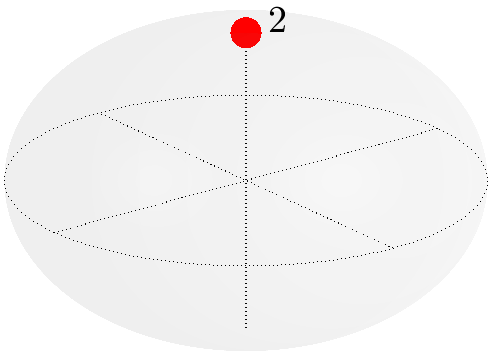
\includegraphics[width=0.3\textwidth]
            {gfx/ch-groundStateSymmetries/FM-Majorana.pdf}};
        \node at (4.5, 0){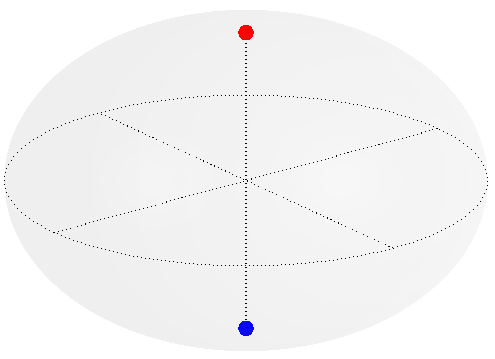
\includegraphics[width=0.3\textwidth]
            {gfx/ch-groundStateSymmetries/polar-Majorana.pdf}};
        \node at (9, 0){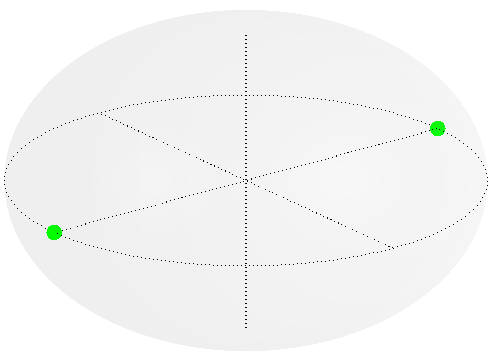
\includegraphics[width=0.3\textwidth]
            {gfx/ch-groundStateSymmetries/AFM-Majorana.pdf}};
        \node at (11.8, 0) {
            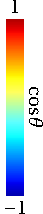
\includegraphics{gfx/colourbars/compiled_jet_majorana.pdf}};

        \node at (0, -2) {(a)};
        \node at (4.5, -2) {(b)};
        \node at (9, -2) {(c)};

        \node at (0, 2) {\(\zeta={(1, 0, 0)}^T\)};
        \node at (4.5, 2) {\(\zeta={(0, 1, 0)}^T\)};
        \node at (9, 2) {\(\zeta={(1, 0, 1)}^T/\sqrt{2}\)};
    \end{tikzpicture}
    \caption[Majorana representation of spin-1 ground states]
    {\label{fig: spin-1-majorana}Majorana representations of spin-1 ground
    states. The colour of the points represent \(\cos\theta =
    (1-|z|^2)/(1+|z|^2)\).
    A number next to a point represents the root when the polynomial
    \(P_\psi^1(z)\) has an \(n\)-multiple root.
    (a): Ferromagnetic state with \(\zeta={(1, 0, 0)}^T\).
    (b): Polar state with \(\zeta={(0, 1, 0)}^T\).
    (c): AFM state with \(\zeta={(1, 0, 1)}^T/\sqrt{2}\).}
\end{figure}

\section{Spin-2}
The interacting Hamiltonian for the spin-2 system is given by
\begin{equation}
    E_\mathrm{int} = \frac{1}{2}\int c_0n^2 + c_1|\vb{F}|^2+c_2|A_{20}|^2
    d\vb{r}.
\end{equation}
As before, the density remains fixed for any normalised ground state and so
different ground states arise from the competition between the spin-
and singlet-dependent interaction strengths.

If we first consider \(c_1 < 0\) and \(c_2 > 0\), then the energy functional is
minimised when  the spin density is maximised \(|F|=2n\)
and the singlet-duo amplitude is minimised \(|A_{20}|=0\).
Such a state is ferromagnetic with spin \(|F|=2n\), which we call the FM-2
state.
There also exists a ferromagnetic state with spin \(|F|=n\), denoted as the FM-1
state.
This state is not the ground state since the FM-2 state has lower
energy.
However, it should be noted that the FM-1 state can remain stable in
certain situations, such as in the cores of vortices (see
Chapter~\ref{chap: spin-2}).
The representative spinors for the spin-2 ferromagnetic states have the form
\begin{equation}
    \zeta^\mathrm{FM-2} = \mqty(1 \\ 0 \\ 0 \\ 0 \\ 0), \qquad
    \zeta^\mathrm{FM-1} = \mqty(0 \\ 1 \\ 0 \\ 0 \\ 0).
\end{equation}

As in the spin-1 case, the energy of a given spinor in the absence of a magnetic
field is degenerate following the application of a global \(U(1)\) phase and an
\(SO(3)\) spin rotation.
In a spin-2 system, a general spin rotation is instead represented as a
\(5\times 5\) matrix of the form
\begin{multline}\label{eq: spin-2-rotation-matrix}
    U(\alpha, \beta, \gamma) = \\
    \scalemath{0.90}{\mqty(
    e^{-2i(\alpha + \gamma)}C^4 & -2e^{-i(2\alpha+\gamma)}C^3S
    & \sqrt{6}e^{-2i\alpha}C^2S^2 & -2e^{-i(2\alpha-\gamma)}CS^3
    & e^{-2i(\alpha + \gamma)}S^4
    \\
    2e^{-i(\alpha+2\gamma)}C^3S & e^{-i(\alpha+\gamma)}C^2(C^2-3S^2)
    & -\sqrt{\frac{3}{8}}e^{-i\alpha}\sin 2\beta
    & -e^{-i(\alpha-\gamma)}S^2(S^2-3C^2) & -2e^{-i(\alpha-2\gamma)}CS^3
    \\
    \sqrt{6}e^{-2i\gamma}C^2S^2 & \sqrt{\frac{3}{8}}e^{-i\gamma}\sin 2\beta
    & \frac{1}{4}(1+3\cos 2\beta)
    & -\sqrt{\frac{3}{8}}e^{-i\gamma}\sin 2\beta
    & \sqrt{6}e^{2i\gamma}C^2S^2
    \\
    2e^{i(\alpha-2\gamma)}CS^3 & -e^{i(\alpha-\gamma)}S^2(S^2-3C^2)
    & \sqrt{\frac{3}{8}}e^{i\alpha}\sin 2\beta
    & e^{i(\alpha-\gamma)}C^2(C^2-3S^2) & -2e^{i(\alpha+2\gamma)}C^3S
    \\
    e^{2i(\alpha - \gamma)}C^4 & 2e^{i(2\alpha-\gamma)}CS^3
    & \sqrt{6}e^{2i\alpha}C^2S^2 & 2e^{i(2\alpha+\gamma)}C^3S
    & e^{2i(\alpha + \gamma)}C^4
    )},
\end{multline}
where \(S \equiv \sin(\beta/2)\) and \(C \equiv \cos(\beta/2)\).

Following the same procedure as the spin-1 case and applying the above spin
rotation with a global phase \(\theta \) and condensate density \(n\) yields the
general FM-2 spinor
\begin{equation}\label{eq: FM-2-representative-spinor}
    \psi^\mathrm{FM} = \sqrt{n}e^{i\theta'}\mqty(
    e^{-2i\alpha} \cos^4\frac{\beta}{2} \\
    2e^{-i\alpha}\cos^3\frac{\beta}{2}\sin \frac{\beta}{2} \\
    \sqrt{6} \cos^2\frac{\beta}{2} \sin^2\frac{\beta}{2} \\
    2e^{i\alpha}\cos\frac{\beta}{2} \sin^3\frac{\beta}{2} \\
    e^{2i\alpha} \sin^4\frac{\beta}{2}
    ),
\end{equation}
where \(\theta'=\theta-2\gamma \).

Instead, let us now consider the case of \(c_1 > 0\) and \(c_2 < 0\).
We see that the energy functional is minimised when the spin is minimised
\(|\vb{F}| = 0\) but the singlet-duo amplitude is maximised
\(|A_{20}|^2 = n/5\).
Such a state is called nematic, and takes two forms: the uniaxial nematic (UN)
or biaxial nematic (BN), described by the spinors
\begin{equation}
    \zeta^\mathrm{UN} = \mqty(0 \\ 0 \\ 1 \\ 0 \\ 0), \qquad
    \zeta^\mathrm{BN} = \frac{1}{\sqrt{2}}\mqty(1 \\ 0 \\0 \\ 0 \\ 1).
\end{equation}
In the absence of a magnetic field, these two states are degenerate.
The general wave function for the UN state is
\begin{equation}\label{eq: UN-representative-spinor}
    \psi^\mathrm{UN} = \frac{\sqrt{6n}}{4}e^{i\theta}\mqty(
    e^{-2i\alpha} \sin^2\beta \\
    -2e^{-i\alpha} \sin\beta \cos\beta \\
    \sqrt{\frac{2}{3}}(3\cos^2\beta - 1) \\
    2e^{i\alpha} \sin\beta \cos\beta \\
    e^{2i\alpha} \sin^2\beta
    ),
\end{equation}
and for the BN
\begin{equation}\label{eq: BN-representative-spinor}
    \psi^\mathrm{BN} = \sqrt{\frac{n}{2}}e^{i\theta} \mqty(
    e^{-2i\alpha}\left[\left(1 - \frac{1}{2}\sin^2\beta\right)\cos 2\gamma
        - i\cos\beta\sin 2\gamma\right] \\
    e^{-i\alpha}\sin\beta(\cos\beta\cos 2\beta - i\sin 2\gamma) \\
    \sqrt{\frac{3}{2}}\sin^2\beta \cos 2\gamma \\
    -e^{i\alpha}\sin\beta(\cos\beta\cos 2\gamma + i\sin 2\gamma) \\
    e^{2i\alpha}\left[\left(1 - \frac{1}{2}\sin^2\beta\right)\cos 2\gamma
        + i\cos\beta\sin 2\gamma\right]
    ).
\end{equation}

Now consider \(c_1, c_2 > 0\).
The energy functional is minimised when both the spin magnitude and singlet-duo
amplitude is minimised: \(|\vb{F}| = 0, |A_{20}|^2=0\).
Such a state is referred to as the cyclic state and has the representative
spinor
\begin{equation}
    \zeta^\mathrm{C-1} = \frac{1}{2}\mqty(1 \\ 0 \\ i\sqrt{2} \\ 0 \\ 1).
    \label{eq: C-1-spinor}
\end{equation}
The general wave function is given as
\begin{equation}
    \psi^\mathrm{C} = \frac{\sqrt{n}}{2}e^{i\theta} \mqty(
    e^{-2i(\alpha+\gamma)}C^4 + 2i\sqrt{3}e^{-2i\alpha}C^2S^2
    + e^{-2i(\alpha-\gamma)}S^4
    \\
    2e^{-i(\alpha+2\gamma)}C^3S - \frac{\sqrt{3}}{2}ie^{-i\alpha}\sin 2\beta
    - 2e^{-i(\alpha-2\gamma)}CS^3
    \\
    \sqrt{6}e^{-2i\gamma}C^2S^2 + i\frac{\sqrt{2}}{4}(1+3\cos 2\beta)
    + \sqrt{6}e^{2i\gamma}C^2S^2
    \\
    2e^{i(\alpha-2\gamma)}CS^3 + \frac{\sqrt{3}}{2}ie^{i\alpha}\sin 2\beta
    - 2e^{i(\alpha+2\gamma)}C^3S
    \\
    e^{2i(\alpha-\gamma)}S^4 + 2i\sqrt{3}e^{2i\alpha}C^2S^2
    + e^{2i(\alpha+\gamma)}C^4
    ).
\end{equation}

In addition to the three-component cyclic state, there is also a two-component
cyclic state that is useful for understanding the general cyclic state:
\begin{equation}
    \zeta^\mathrm{C-2} = \frac{1}{\sqrt{3}}\mqty(1  \\ 0 \\ 0 \\ \sqrt{2} \\ 0),
    \label{eq: C-2-spinor}
\end{equation}
which is obtained from Eq.~\eqref{eq: C-1-spinor} via the spin rotation
\begin{equation}
    \zeta^{C-2} = e^{-i\pi}e^{i\frac{\pi}{4}F_z}
    \exp\left[-i\frac{F_x-F_y}{\sqrt{2}}
        \arccos{\left(\frac{1}{\sqrt{3}}\right)}\right]\zeta^\mathrm{C-1}.
\end{equation}

Finally, for the case of \(c_1, c_2 < 0\), there is a competition between
the ferromagnetic and nematic phases.
For this case the energy functional is minimised by either having maximal spin
density and \(|A_{20}|^2 = 0\) as in the ferromagnetic phase, or by having
minimal spin density and \(|A_{20}|^2 = n/5\) as in the nematic phase.
This leads to a phase boundary at \(c_2n=20c_1n\).
The ground states of the spin-2 system in a parameter space of \((c_1, c_2)\)
are summarised in Fig.~\ref{fig: spin-2-ground-states}.
\begin{figure}
    \centering
    \begin{tikzpicture}
        \node[anchor=south west, inner sep=0] (diagram) at (0, 0)
        {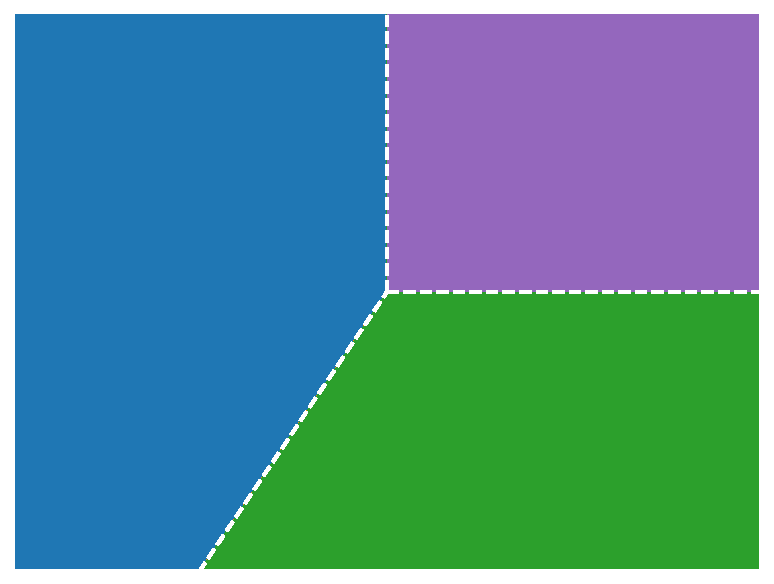
\includegraphics[width=0.5\textwidth]
            {gfx/ch-groundStateSymmetries/ground_states_spin2.pdf}};
        \begin{scope}[x={($0.1*(diagram.south east)$)},
                y={($0.1*(diagram.north west)$)}]
            \draw[->, thick, anchor=south west] (9.8, 5) -- (10.1, 5)
            node[right] {$c_1n$};
            \draw[->, thick, anchor=south west] (5, 9.7) -- (5, 10.1)
            node[above] {$c_2n$};
            \draw[-, thick, anchor=south west] (0.21, 5) -- (4.98, 5);
            \node at (7.5, 7) {\textcolor{white}{Cyclic}};
            \node at (2.5, 7) {\textcolor{white}{Ferromagnetic}};
            \node at (7, 2) {\textcolor{white}{Nematic}};
            \node[anchor=south east] at (5, 5) {\textcolor{white}{0}};
            \node[anchor=south west, rotate=53] at (2.7, 0.7)
            {\textcolor{white}{\(c_2n=20c_1n\)}};
        \end{scope}
    \end{tikzpicture}
    \caption[Spin-2 ground state phase diagram]
    {\label{fig: spin-2-ground-states}Ground state phase diagram for
        spin-2 BECs in a parameter space of \((c_1, c_2)\) in the absence of a
        magnetic field.
        White dashed lines indicate a first-order phase transition region
        between the phases.}
\end{figure}

\subsection{Graphical representation}
The mapping of the order parameter onto spherical harmonics in the spin-2 case
follows the same equation as in the spin-1 case, i.e.,
Eq.~\eqref{eq: spherical-harmonics}.
For the spin-2 system, however, we have five \(f=2\) spherical harmonics given
by
\begin{align}
    Y_2^0(\theta, \phi)       & = \frac{1}{4}\sqrt{\frac{5}{\pi}}
    (3\cos^2\theta - 1),                                                    \\
    Y_2^{\pm 1}(\theta, \phi) & =
    \mp \frac{1}{2}\sqrt{\frac{15}{2\pi}}e^{\pm i\phi}\sin\theta\cos\theta, \\
    Y_2^{\pm 2}(\theta, \phi) & =
    \frac{1}{4}\sqrt{\frac{15}{2\pi}}e^{\pm 2i\phi}\sin^2\theta.
\end{align}
The spherical harmonics for the ferromagnetic, UN, BN, and cyclic states
are shown in Fig.~\ref{fig: spin-2-spherical-harmonics}.
\begin{figure}
    \centering
    \begin{tikzpicture}
        % Plots
        \node at (0, 0) {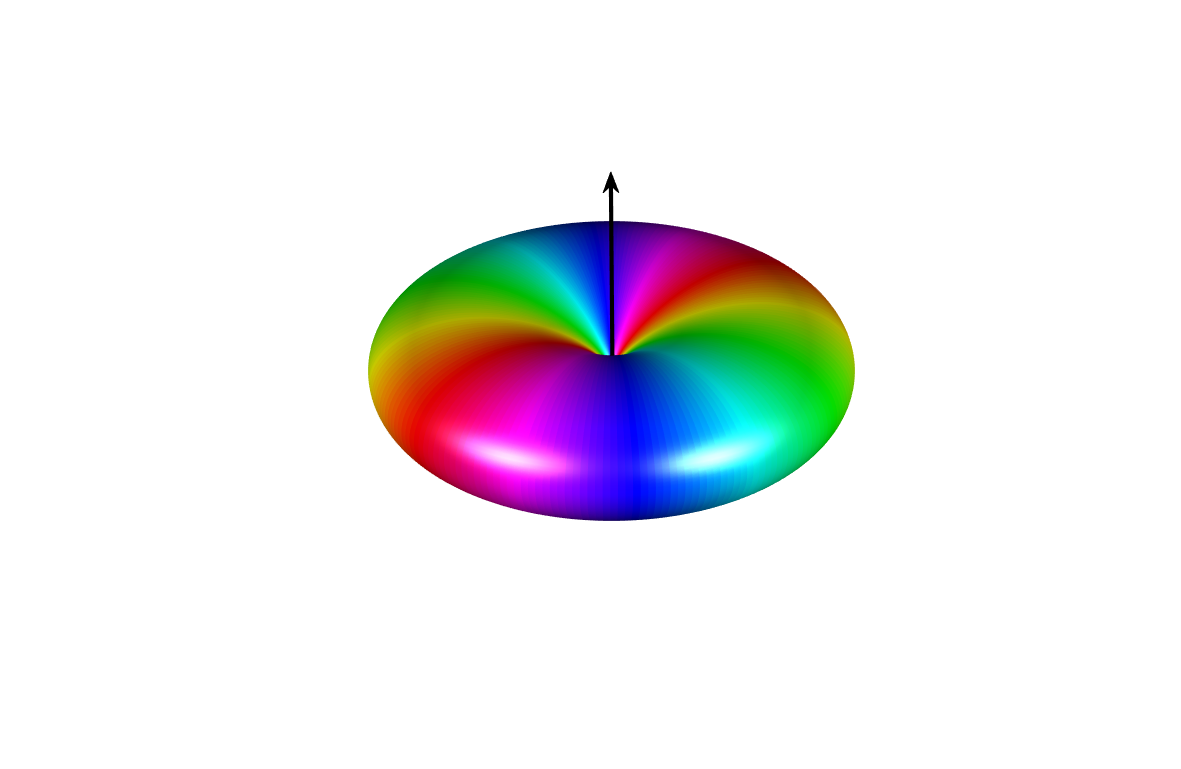
\includegraphics[width=0.45\textwidth]
            {gfx/ch-groundStateSymmetries/FM-2-spherical.pdf}};
        \node at (7.2, 0) {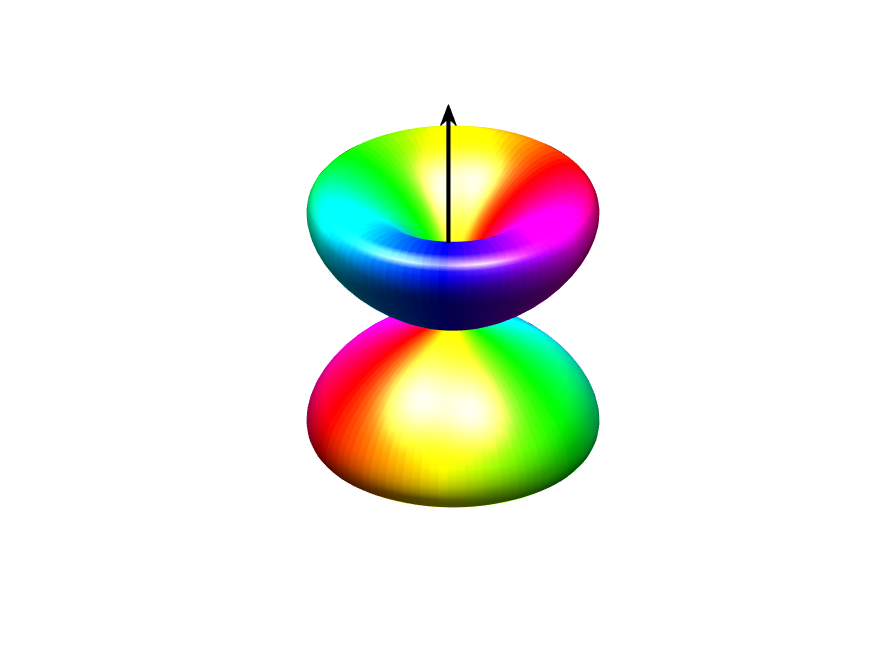
\includegraphics[width=0.45\textwidth]
            {gfx/ch-groundStateSymmetries/FM-1-spherical.pdf}};
        \node at (0, -6) {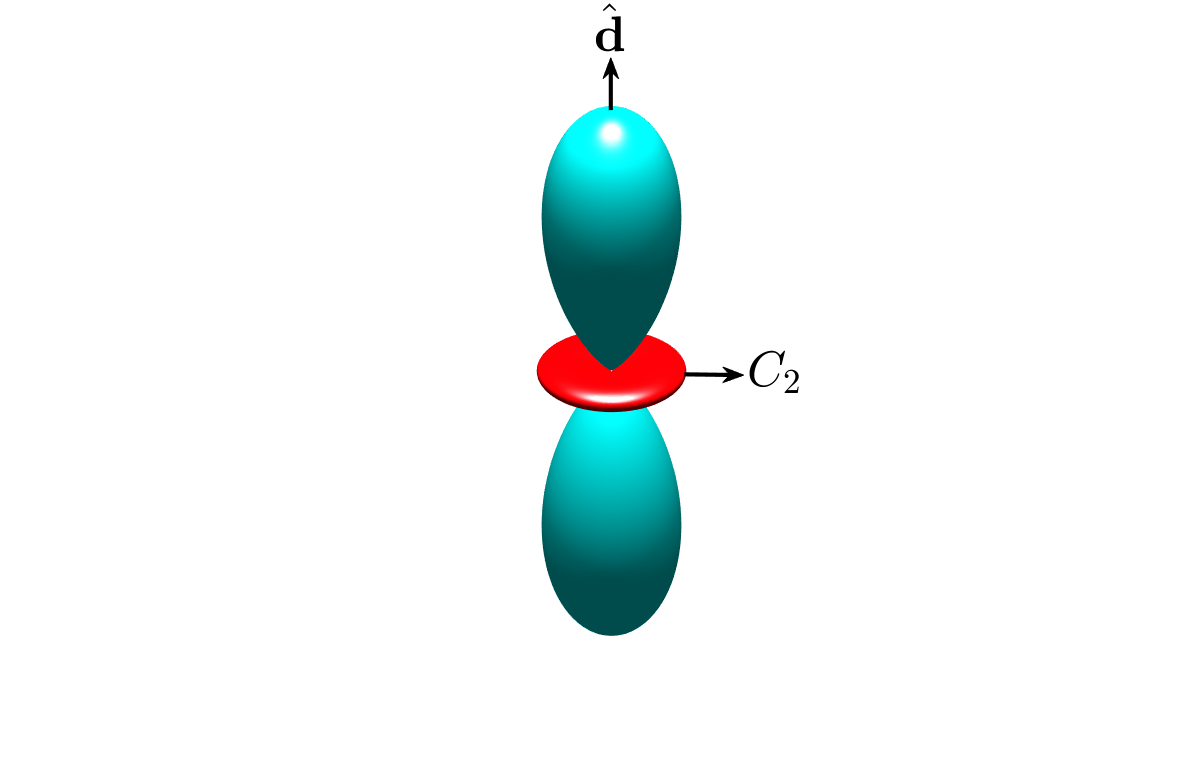
\includegraphics[width=0.45\textwidth]
            {gfx/ch-groundStateSymmetries/UN-spherical.pdf}};
        \node at (7.2, -6) {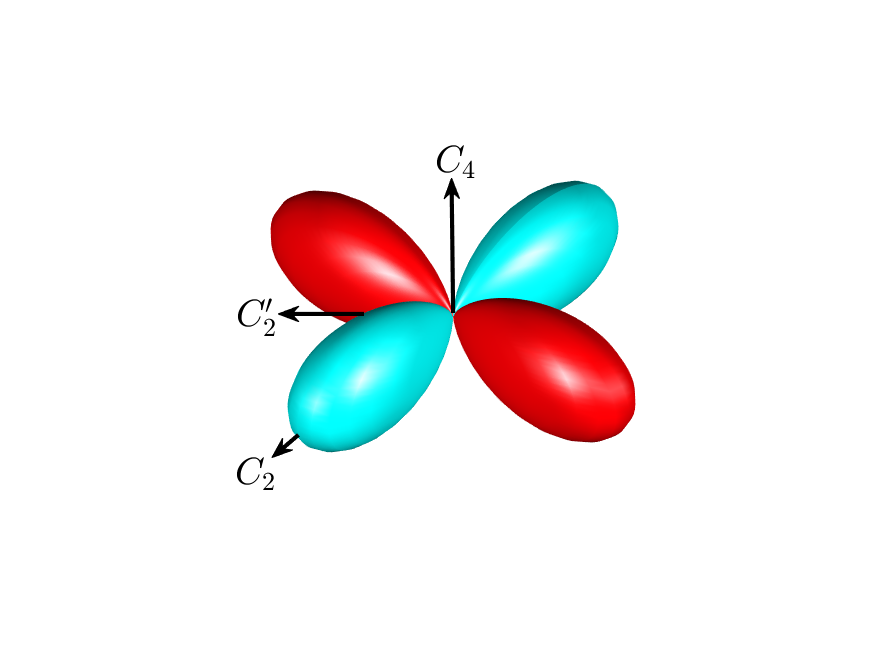
\includegraphics[width=0.45\textwidth]
            {gfx/ch-groundStateSymmetries/BN-spherical.pdf}};
        \node at (0, -12) {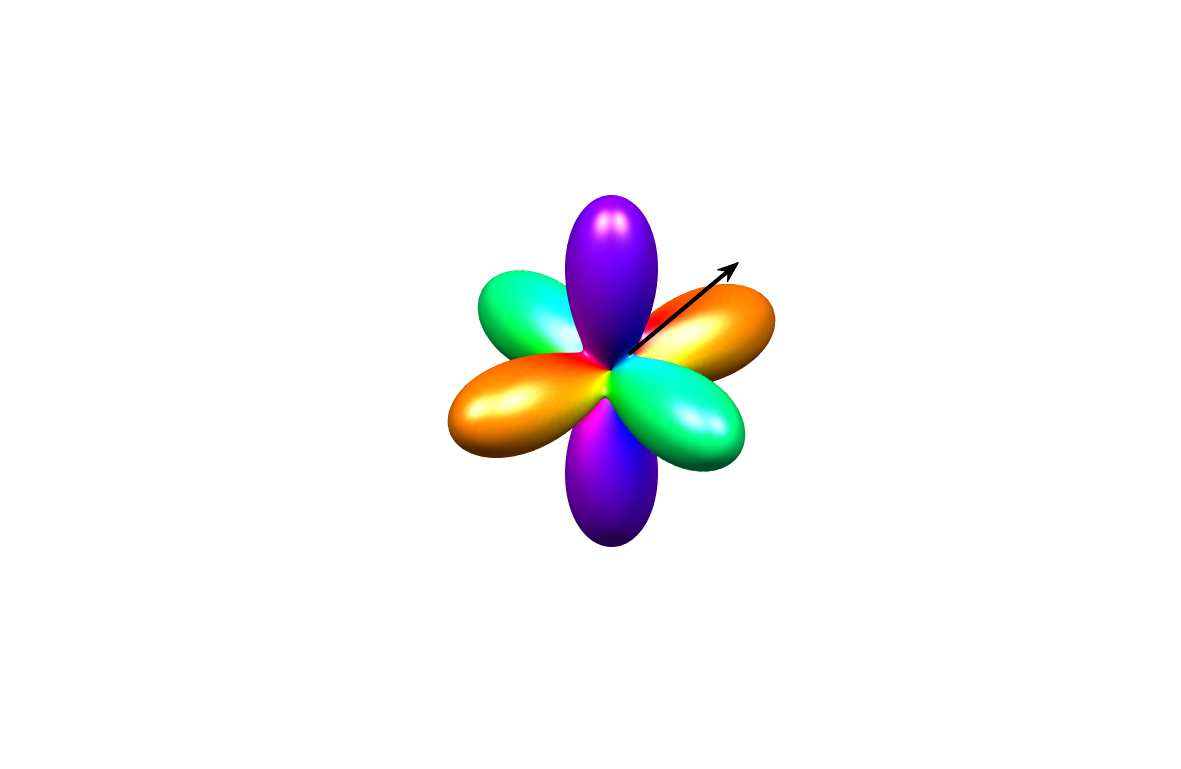
\includegraphics[width=0.45\textwidth]
            {gfx/ch-groundStateSymmetries/C1-spherical.pdf}};
        \node at (7.2, -12) {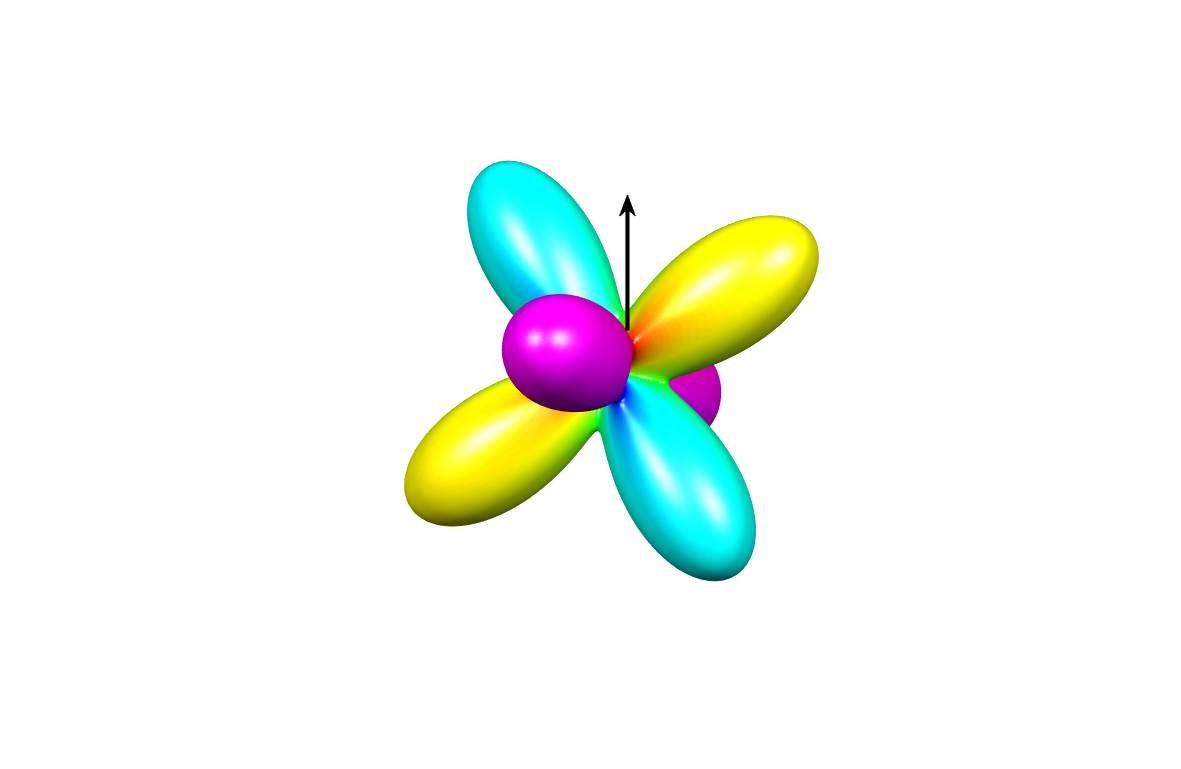
\includegraphics[width=0.45\textwidth]
            {gfx/ch-groundStateSymmetries/C2-spherical.pdf}};

        % Colour bars
        \node at (3.2, -13.6) {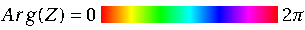
\includegraphics{gfx/colourbars/compiled_hsv.pdf}};

        % Labels
        \node at (0, -2) {(a)};
        \node at (7.2, -2) {(b)};
        \node at (0, -8) {(c)};
        \node at (7.2, -8) {(d)};
        \node at (0, -14) {(e)};
        \node at (7.2, -14) {(f)};

        % Spinors
        \node at (0, 2.5) {\(\zeta={(1, 0, 0, 0, 0)}^T\)};
        \node at (7.2, 2.5) {\(\zeta={(0, 1, 0, 0, 0)}^T\)};
        \node at (0, -3.2) {\(\zeta={(0, 0, 1, 0, 0)}^T\)};
        \node at (7.2, -3.2) {\(\zeta={(1, 0, 0, 0, 1)}^T/\sqrt{2}\)};
        \node at (0, -9.5) {\(\zeta={(1, 0, i\sqrt{2}, 0, 1)}^T/2\)};
        \node at (7.2, -9.5) {\(\zeta={(\sqrt{1/3}, 0, 0, \sqrt{2/3}, 0)}^T\)};
    \end{tikzpicture}
    \caption[Spherical harmonic representation of spin-2 ground states]
    {\label{fig: spin-2-spherical-harmonics}Spherical harmonic
        representations for different ground states in a spin-2 system.
        (a) and (b): Ferromagnetic states with a spin of \(|F|=2n\) and
        \(|F|=n\), respectively, where the arrows indicate the direction of
        magnetisation.
        (c): the uniaxial nematic state where \(\hat{\vb{d}}\) is the nematic
        director. The order parameter remains unchanged about \(\pi \) rotations
        about the \(C_2\) axis.
        (d): the biaxial nematic state. The order parameter is symmetric under
        \(\pi/2\) rotations about the \(C_4\) axis.
        Additionally, there is a two-fold symmetry about the \(C_2, C_2'\) axes.
        (e) and (f): the cyclic states which have a two- and three-fold symmetry
        about the \(C_2, C_3\) axes, respectively.
    }
\end{figure}

It is clear from Figs~\ref{fig: spin-2-spherical-harmonics}a
and~\ref{fig: spin-2-spherical-harmonics}b that the ferromagnetic order
parameters have the same \(SO(2)\) symmetry about the \(z\)-axis as the spin-1
case.
However, the difference between the FM-2 phase of the spin-2 system and the FM
phase of the spin-1 system is apparent in the phase: the FM-2 state winds by
\(4\pi \) about the spherical harmonic as opposed to \(2\pi \)
(see Fig.~\ref{fig: spin-1-spherical-harmonics}a).

The UN phase as shown in Fig.~\ref{fig: spin-2-spherical-harmonics}c differs
slightly from the polar phase of spin-1 (see
Fig.~\ref{fig: spin-1-spherical-harmonics}b) in that the nematic lobes have the
same phase.
This implies that a \(\pi \) spin rotation about any axis in the \(xy\)-plane
leaves the order parameter unchanged.
In addition, like the ferromagnetic states, this order parameter also has an
\(SO(2)\) symmetry about the \(z\)-axis.

The BN phase, shown in Fig.~\ref{fig: spin-2-spherical-harmonics}d, breaks the
\(SO(2)\) symmetry due to the perpendicular nematic lobes, which have a \(\pi \)
phase difference.
The symmetry of the order parameter is preserved under \(\pi/4\) rotations
about the \(C_4\) axis.
In addition, the BN order parameter is invariant under \(\pi \) rotations about
both the \(C_2\) and \(C_2'\) axes.

Finally, the cyclic order parameter, shown in
Figs.~\ref{fig: spin-2-spherical-harmonics}e
and~\ref{fig: spin-2-spherical-harmonics}f, have the symmetry of a tetrahedron.
Each nematic lobe has a two-fold symmetry about the \(C_2\) axis.
Furthermore, the order parameter has a three-fold symmetry about the \(C_3\)
axis.
In Fig.~\ref{fig: spin-2-spherical-harmonics}e, this axis is the
\((1, 1, 1)\)-axis, whereas in Fig.~\ref{fig: spin-2-spherical-harmonics}f,
it is aligned along the \(z\)-axis.
Rotations of \(2\pi/3\) about this axis preserve the symmetry of the order
parameter.

The mapping of the spin-2 system onto the Majorana representation follows a
similar procedure to the spin-1 case.
In this system, we compute the \(2f=4\) roots of the complex polynomial
\begin{equation}
    P^{(2)}(z) = \zeta_2^*z^4 + 2\zeta_1^*z^3 + \sqrt{6}\zeta_0^*z^2
    + 2\zeta_{-1}^*z + \zeta_{-2}^*.
\end{equation}
The Majorana representation of the ferromagnetic, UN, BN, and cyclic states
are shown in Fig.~\ref{fig: spin-2-Majorana}.
\begin{figure}
    \centering
    \begin{tikzpicture}
        % First row
        \node at (0, 0){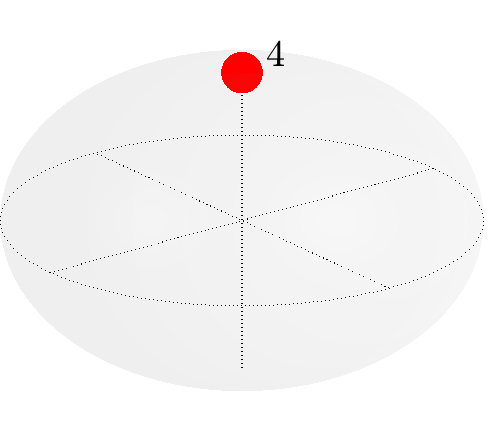
\includegraphics[width=0.3\textwidth]
            {gfx/ch-groundStateSymmetries/FM-2-Majorana.pdf}};
        \node at (4.5, 0){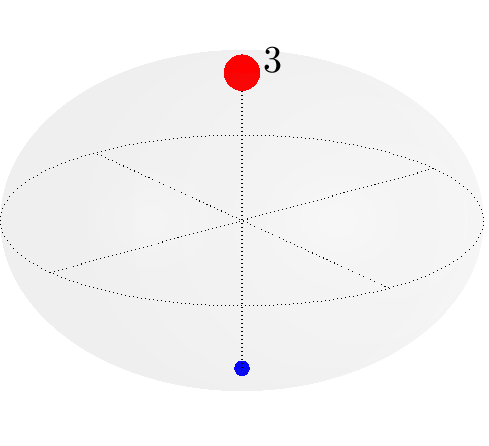
\includegraphics[width=0.3\textwidth]
            {gfx/ch-groundStateSymmetries/FM-1-Majorana.pdf}};
        \node at (9, 0){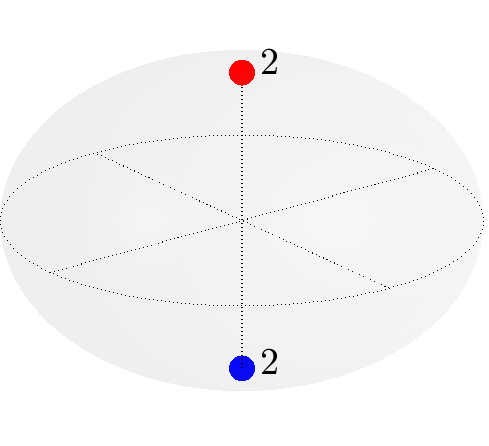
\includegraphics[width=0.3\textwidth]
            {gfx/ch-groundStateSymmetries/UN-Majorana.pdf}};
        \node at (11.8, -2.5) {
            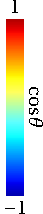
\includegraphics{gfx/colourbars/compiled_jet_majorana.pdf}};

        \node at (0, -2) {(a)};
        \node at (4.5, -2) {(b)};
        \node at (9, -2) {(c)};

        \node at (0, 2) {\(\zeta={(1, 0, 0, 0, 0)}^T\)};
        \node at (4.5, 2) {\(\zeta={(0, 1, 0, 0, 0)}^T\)};
        \node at (9, 2) {\(\zeta={(0, 0, 1, 0, 0)}^T\)};

        % Second row
        \node at (0, -5){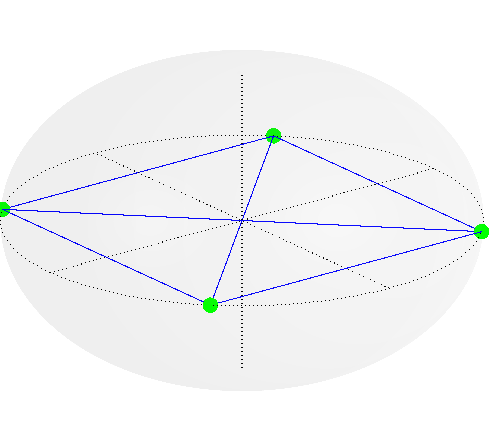
\includegraphics[width=0.3\textwidth]
            {gfx/ch-groundStateSymmetries/BN-Majorana.pdf}};
        \node at (4.5, -5){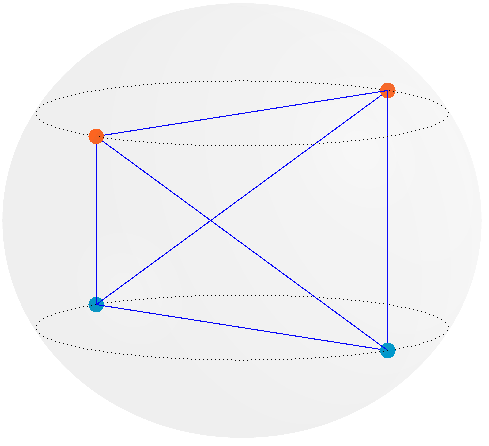
\includegraphics[width=0.265\textwidth]
            {gfx/ch-groundStateSymmetries/C1-Majorana.pdf}};
        \node at (9, -5){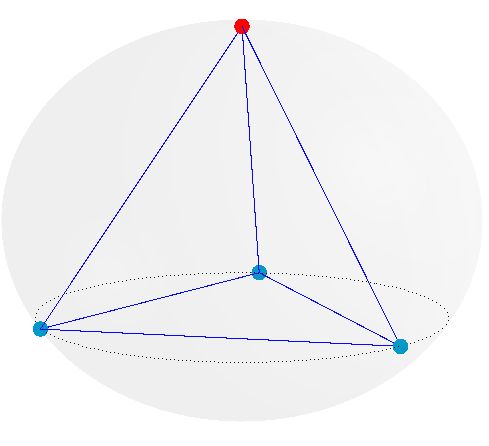
\includegraphics[width=0.275\textwidth]
            {gfx/ch-groundStateSymmetries/C2-Majorana.pdf}};

        \node at (0, -7) {(d)};
        \node at (4.5, -7) {(e)};
        \node at (9, -7) {(f)};

        \node at (0, -3) {\(\zeta={(1, 0, 0, 0, 1)}^T/\sqrt{2}\)};
        \node at (4.5, -3) {\(\zeta={(1, 0, i\sqrt{2}, 0, 1)}^T/2\)};
        \node at (9, -3) {\(\zeta={(\sqrt{1/3}, 0, 0, \sqrt{2/3}, 0)}^T\)};
    \end{tikzpicture}
    \caption[Majorana representation of spin-2 ground states]
    {\label{fig: spin-2-Majorana}Majorana representation of spin-2 ground
    states.
    As in the spin-1 case, the colour of the points represent \(\cos\theta =
    (1-|z|^2)/(1+|z|^2)\), whilst a number next to a point represents the root
    when the polynomial \(P_\psi^1(z)\) has an \(n\)-multiple root.
    (a): FM-2 state with \(\zeta={(1, 0, 0, 0, 0)}^T\).
    (b): FM-1 state with \(\zeta={(0, 1, 0, 0, 0)}^T\).
    (c): UN state with \(\zeta={(0, 0, 1, 0, 0)}^T\).
    (d): BN state with \(\zeta={(1, 0, 0, 0, 1)}^T/\sqrt{2}\).
    (e): Three-component cyclic state with
    \(\zeta={(1, 0, i\sqrt{2}, 0, i)}^T/2\).
    (f): Two-component cyclic state with
    \(\zeta={(\sqrt{1/3}, 0, 0, \sqrt{2/3}, 0)}^T\).}
\end{figure}

\section{Topological defects in spinor BECs}
Unlike scalar BECs, which only support a \(U(1)\) vortex, spinor BECs have a
rich diagram of vortices.
Generally, the properties of vortices are determined by visualising how the
order parameter changes around a closed loop about the vortex.
In a scalar BEC, the single-value condition of the wave function is satisfied
by having the density vanish along the core.
In a spinor system, however, the condition can instead be satisfied by lifting
the system out of the ground state within the vortex core.
This leads to novel vortices such as fractional vortices in the
cyclic~\cite{Semenoff2007,Huhtamaki2009} and nematic
phases~\cite{Leonhardt2000, Seo2015}.
In this section we introduce some families of vortices that can occur
in both spin-1 and spin-2 systems.

\subsection{Spin-1}\label{sec: vortices-spin-1}
We start with the polar phase of a spin-1 condensate, with the representative
spinor defined as in Eq.~\eqref{eq: polar-representative-spinor}.
Unlike the scalar BEC, a singly quantised vortex in the polar phase does not
represent the lowest unit of circulation.
Instead, the polar phase allows for a vortex where the global phase only winds
by \(\pi \) about the vortex core.
This \(\pi \) rotation is then coupled with a \(\pi \) spin rotation to the
nematic director \(\hat{\vb{d}}\) to keep the order parameter single valued.

If we consider a vortex that is oriented along the \(z\)-axis and the nematic
director is oriented in the \((x, y)\)-plane, then such a vortex corresponds to
the choice of \(\theta=\alpha=\varphi/2 \) and \(\beta = \pi/2\) in
Eq.~\eqref{eq: polar-representative-spinor} to yield the wave function
\begin{equation}
    \psi^\mathrm{HQV} = \sqrt{\frac{n}{2}} \mqty(
    -1 \\
    0 \\
    e^{i\varphi}
    ),
    \label{eq: polar-HQV}
\end{equation}
where \(\varphi \) is the azimuthal angle about the vortex core.
Such a vortex is referred to as a half-quantum vortex (HQV) due to carrying
half the typical circulation of a scalar \(U(1)\) vortex.
Similar, but topologically distinct vortices arise in the A phase of
superfluid \( ^3\)He~\cite{Salomaa1985, Salomaa1987}.

In experiment, for the vortex constructed as in Eq.~\eqref{eq: polar-HQV}, the
vortex consists of density depletion along the core in the \(\psi_{-1}\)
component, where the phase winding is located.
This core is then filled with atoms of the \(\psi_1 \) component, which lifts
the core out of the polar phase and into the ferromagnetic phase.
Fig.~\ref{fig: spin-1-vortices}a shows the spherical harmonic representation of
the HQV\@.
\begin{figure}
    \centering
    \begin{tikzpicture}
        \node at (0, 0) {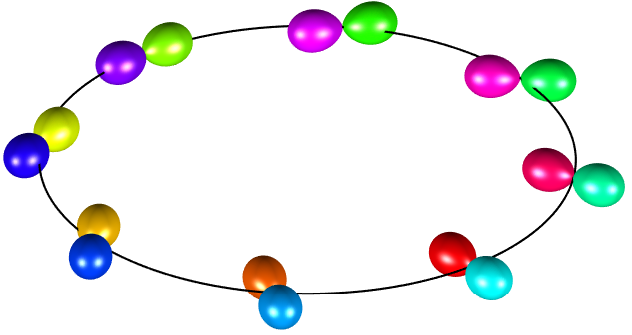
\includegraphics[width=0.45\textwidth]
            {gfx/ch-groundStateSymmetries/polar-HQV.pdf}};
        \node at (7.2, 0) {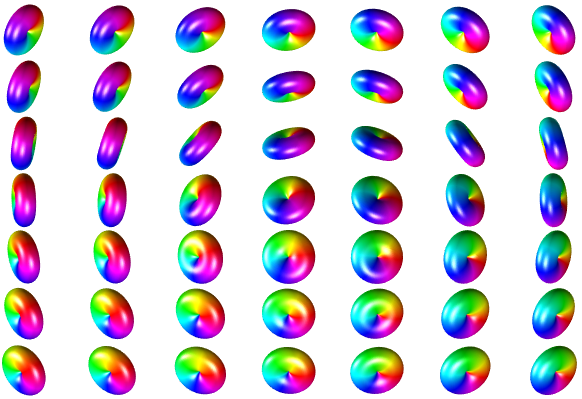
\includegraphics[width=0.45\textwidth]
            {gfx/ch-groundStateSymmetries/coreless.pdf}};
        \node at (-3.6, -0.2) {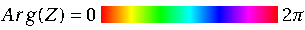
\includegraphics[angle=90]
            {gfx/colourbars/compiled_hsv.pdf}};

        % Labels
        \node at (0, -3) {(a)};
        \node at (7.2, -3) {(b)};
    \end{tikzpicture}
    \caption[Spherical harmonic representation of spin-1 vortices]
    {\label{fig: spin-1-vortices}Spherical harmonic representation of vortices
        in a spin-1 BEC\@.
        (a): Spin-1 polar HQV defined by Eq.~\eqref{eq: polar-HQV}.
        A complete circuit of the vortex results in a \(\pi \) spin rotation of
        the nematic director coupled with a \(\pi \) change to the condensate
        phase.
        (b): Ferromagnetic coreless vortex.
        The vortex takes on a characteristic fountain-like texture of the
        condensate spin vector.
    }
\end{figure}

The ferromagnetic phase has the unique property that circulation is not
quantised~\cite{Kawaguchi2012}.
This leads to both singular and non-singular defects present in this phase.
Here, we discuss a particular type of non-singular vortex called the coreless
vortex~\cite{Martikainen2002, Leanhardt2003}.

From Eq.~\eqref{eq: FM-representative-spinor}, a coreless vortex is constructed
using the choice of \(\theta-\gamma = \alpha= \varphi \) and having
\(\beta = \beta(\rho)\) be a function of the radial coordinate, \(\rho \):
\begin{equation}
    \psi^\mathrm{coreless} = \sqrt{n}\mqty(
    \cos^2\frac{\beta}{2} \\
    \frac{e^{i\varphi}}{\sqrt{2}}\sin\beta \\
    e^{2i\varphi}\sin^2\frac{\beta}{2}
    ).
\end{equation}
The single-valued condition of the wave function is satisfied by choosing
\(\beta \) such that \(\beta(r=0) = 0\) and \(\beta(r=r_0) = \pi \), where
\(r_0\) is the radius of the system.
This choice of \(\beta \) results in a vortex-free configuration at \(r=0\),
which then terminates on a doubly-quantised vortex at \(r=r_0\).
A spherical harmonic representation of the coreless vortex is shown in
Fig.~\ref{fig: spin-1-vortices}b, where the characteristic fountain-like
spin texture is apparent.

\subsection{Spin-2}\label{sec: vortices-spin-2}
Spin-2 BECs offer an even richer diagram of topological defects than their
spin-1 counterparts.
We start with the UN phase, as given by
Eq.~\eqref{eq: UN-representative-spinor}.
Unlike the spin-1 polar phase, the UN phase does not support fractional vortices
with mass circulation.
This is apparent from the spherical harmonic representation given in
Fig.~\ref{fig: spin-2-spherical-harmonics}c, where the \(\mathbb{Z}_2\) symmetry
about the \(C_2\) axis is not coupled to the condensate phase, \(\theta \).
This phase instead accommodates a spin vortex, i.e., a vortex which carries only
spin circulation.
Such a vortex is constructed from Eq.~\eqref{eq: UN-representative-spinor} with
the choice \(\theta=0, \alpha=-\varphi/2, \beta=\pi/2\):
\begin{equation}
    \psi^\mathrm{SV} = \frac{\sqrt{6n}}{4}\mqty(
    e^{i\varphi} \\
    0 \\
    -\sqrt{\frac{2}{3}} \\
    0 \\ e^{-i\varphi}
    ).
\end{equation}
The spherical harmonic representation of this vortex state is shown in
Fig.~\ref{fig: SV-HQV}a.
\begin{figure}
    \centering
    \begin{tikzpicture}
        \node at (0, 0) {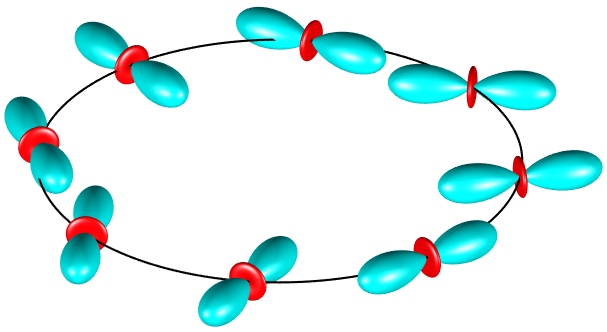
\includegraphics[width=0.45\textwidth]
            {gfx/ch-groundStateSymmetries/UN-spin-vortex.pdf}};
        \node at (7.3, 0) {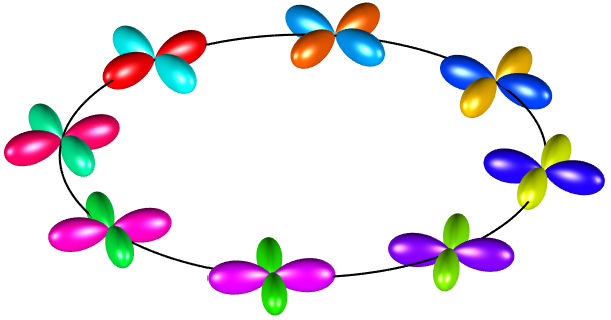
\includegraphics[width=0.45\textwidth]
            {gfx/ch-groundStateSymmetries/BN-HQV.pdf}};
        \node at (3.0, -2) {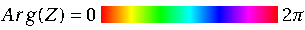
\includegraphics{gfx/colourbars/compiled_hsv.pdf}};

        % Labels
        \node at (-0.8, -2.2) {(a)};
        \node at (7.2, -2.2) {(b)};
    \end{tikzpicture}
    \caption[Spherical harmonic representation of spin-2 vortices]
    {\label{fig: SV-HQV}Spherical harmonic representation of select vortices in the spin-2
        nematic phases.
        (a): A spin vortex in the UN phase. A complete circuit of the vortex
        results in a \(\pi \) winding of the condensate spin vector, with no
        change to the condensate phase.
        (b): One type of half-quantum vortex in the BN phase.
        The condensate phase winds by \(\pi \) about the vortex core which is
        coupled to a \(\pi / 2\) spin rotation.}
\end{figure}
As the core of the vortex is traversed, the spin vector winds by \(\pi \) about
the axis perpendicular to the nematic director, \(\hat{\vb{d}}\).

The BN phase is the simplest order parameter that supports non-abelian defects,
i.e., defects whose topological charges do not commute~\cite{Mermin1979}.
One of the simplest defects in this phase is the half-quantum vortex.
However, this is topologically distinct from that of the spin-1 polar case.
Such a vortex can be constructed from Eq.~\eqref{eq: BN-representative-spinor}
using the choice \(\theta=2\alpha=\varphi/2\) and \(\beta=\gamma=0\):
\begin{equation}
    \psi^\mathrm{1/2-1/4} = \sqrt{\frac{n}{2}}\mqty(
    1 \\
    0 \\
    0 \\
    0 \\
    e^{i\varphi}
    ).
\end{equation}
The spherical harmonic representation of this vortex is shown in
Fig.~\ref{fig: SV-HQV}b.
It is the clear the condensate phase winds by \(\pi \) about the vortex core,
which is also coupled to a \(\pi / 2\) spin rotation.
This configuration is sometimes denoted a \(1/2-1/4\) vortex, where the \(1/2\)
and \(1/4\) denote the phase and spin rotation angles, respectively.

This is not the only type of HQV that the BN phase supports.
For example, there exists a pure spin vortex (\(0 - 1/2\) vortex) and a HQV
that is also coupled to a \(\pi \) spin rotation
(\(1/2-1/2\) vortex)~\cite{Kawaguchi2012}.

Finally, the cyclic phase also allows for fractional vortices.
However, the circulation in this phase is quantised in units of \(\kappa / 3\),
leading to \(1/3\) and \(2/3\) vortices.
These vortices are constructed by applying a condensate phase and general spin
rotation to Eq.~\eqref{eq: C-2-spinor}.
A \(1/3\) vortex is constructed from the choice
\(\theta = -\alpha = \varphi/3 \) with \(\gamma = 0\).
Similarly, a \(2/3\) vortex is constructed by choosing \(\theta = 2\varphi/3\),
\(\alpha = \varphi/3\) and \(\gamma=0\).
The result is a phase winding in the \(\psi_2\) and \(\psi_{-1}\) components
for the \(1/3\) and \(2/3\) vortices, respectively:
\begin{equation}
    \psi^{1/3} = \sqrt{\frac{n}{3}}\mqty(e^{i\varphi} \\ 0 \\ 0 \\ \sqrt{2}\\0),
    \qquad
    \psi^{2/3} = \sqrt{\frac{n}{3}}\mqty(1 \\ 0 \\ 0 \\\sqrt{2}e^{i\varphi}\\0).
\end{equation}
Spherical harmonic representations are plotted in
Fig.~\ref{fig: cyclic-fractional-spherical}.
\begin{figure}
    \centering
    \begin{tikzpicture}
        \node at (0, 0) {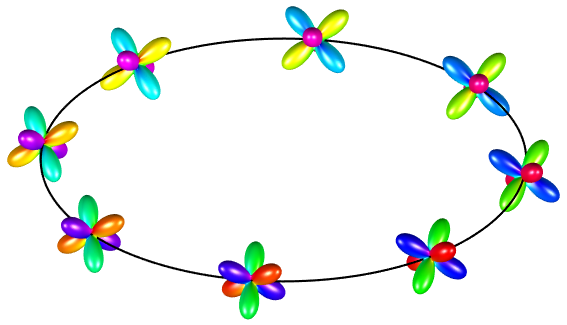
\includegraphics[width=0.45\textwidth]
            {gfx/ch-groundStateSymmetries/one-third-vortex.pdf}};
        \node at (7.3, 0) {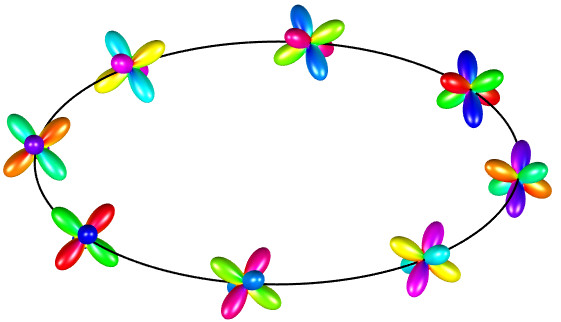
\includegraphics[width=0.45\textwidth]
            {gfx/ch-groundStateSymmetries/two-third-vortex.pdf}};
        \node at (3, -2) {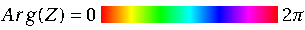
\includegraphics{gfx/colourbars/compiled_hsv.pdf}};

        \node at (0, -2.2) {(a)};
        \node at (7.2, -2.2) {(b)};
    \end{tikzpicture}
    \caption[Spherical harmonic representation of cyclic fractional vortices]
    {\label{fig: cyclic-fractional-spherical}Spherical harmonic
        representations of cyclic fractional vortices.
        (a): The \(\frac{1}{3}\) vortex. A complete circuit reveals a \(2\pi/3\)
        winding of the condensate phase, coupled with a \(\pi/2\) spin rotation.
        (b): The \(\frac{2}{3}\) vortex. Similarly, a complete circuit of the
        vortex results in a \(4\pi/3\) winding of the condensate phase, again
        coupled to a \(\pi/2\) spin rotation.}
\end{figure}
